%%%%%%%%%%%%%%%%%%%%%%%%%%%%%%%%%%%%%%%%%%%%%%%%%%%
%
%  New template code for TAMU Theses and Dissertations starting Fall 2012.  
%  For more info about this template or the 
%  TAMU LaTeX User's Group, see http://www.howdy.me/.
%
%  Author: Wendy Lynn Turner 
%	 Version 1.0 
%  Last updated 8/5/2012
%
%%%%%%%%%%%%%%%%%%%%%%%%%%%%%%%%%%%%%%%%%%%%%%%%%%%

%%%%%%%%%%%%%%%%%%%%%%%%%%%%%%%%%%%%%%%%%%%%%%%%%%%%%%%%%%%%%%%%%%%%%%
%%                           APPENDIX - DSA
%%%%%%%%%%%%%%%%%%%%%%%%%%%%%%%%%%%%%%%%%%%%%%%%%%%%%%%%%%%%%%%%%%%%%

\chapter{\uppercase {Addendum to Chapter \ref{sec::DSA}}}
\label{sec::appendix_DSA}

In this appendix, we will perform some additional analysis of the MIP diffusion form. First, we provide greater implementation details for Fourier Analysis in Section \ref{sec::App_DSA_fourier}. Then, we conclude with some example Fourier Analysis for the 1D MIP DSA scheme in Section \ref{sec::App_DSA_resutls}.

%%%%%%%%%%%%%%%%%%%%%%%%%%%%%%%%%%%%%%%%%%%%%%%%%%%
%%%%%%%%%%%%%%%%%%%%%%%%%%%%%%%%%%%%%%%%%%%%%%%%%%%
%%%   Section - 1D
%%%%%%%%%%%%%%%%%%%%%%%%%%%%%%%%%%%%%%%%%%%%%%%%%%%
%%%%%%%%%%%%%%%%%%%%%%%%%%%%%%%%%%%%%%%%%%%%%%%%%%%
\section{Extended Fourier Analysis Implementation for MIP in 1D}
\label{sec::App_DSA_fourier}

In this section, we give greater detail on how to implement discretized Fourier Analysis through the use of a 1D example.

\begin{equation}
\label{eq::App_DSA_1D_transport_eq}
\mu \frac{d }{d x} \psi (x,\mu) + \sigma_t (x) \psi(x,\mu) = \int\limits_{-1}^{1} d\mu'  \, \sigma_s (x) \psi(x,\mu') + \frac{Q(x)}{2}
\end{equation}

\noindent If we define a 1D angular quadrature, $\{  \mu_m, w_m \}_{m=1}^M$, suppress the spatial and angular parameters and apply SI, we can rewrite Eq. (\ref{eq::App_DSA_1D_transport_eq}) into

\begin{equation}
\label{eq::App_DSA_1D_transport_discangle}
\begin{aligned}
\mu_m \frac{d }{d x} \psi_m^{(k+1/2)} + \sigma_t \psi_m^{(k+1/2)} &= \frac{\sigma_s}{2} \sum_{m=1}^M w_m \psi_m^{(k)} + \frac{Q}{2} \\
&= \frac{\sigma_s }{2} \phi^{(k)}  + \frac{Q}{2}
\end{aligned} ,
\end{equation}

\noindent where

\begin{equation}
\label{eq::App_DSA_1D_angint}
\phi^{(k)} = \sum_{m=1}^M w_m \psi_m^{(k)},
\end{equation}

\noindent and we assume constant cross sections and a constant isotropic source.

\begin{equation}
\label{eq::App_DSA_1D_transport_ops}
{\bf L} \Psi^{(k+1/2)} = {\bf M} {\bf S} \Phi^{(k)}  + {\bf Q}
\end{equation}

\begin{equation}
\label{eq::App_DSA_1D_diff_eq}
- \frac{d}{dx} D \frac{d }{dx} \delta \phi^{(k+1/2)}+ \sigma_a \delta \phi^{(k+1/2)} = \sigma_s \left(  \phi^{(k+1/2)} - \phi^{(k)} \right)
\end{equation}

\begin{equation}
\label{eq::App_DSA_1D_diff_ops}
{\bf A} \Phi^{(k+1/2)} = {\bf S}\left( \Phi^{(k+1/2)} -  \Phi^{(k)}   \right)
\end{equation}

Using the 1D LD basis functions, the cell-wise elementary matrices for the mass, stiffness, and gradient matrices for a cell of width $h$ are

\begin{equation}
\label{eq::App_DSA_MIP_1D_cell_matrices}
\begin{aligned}
	\mathbb{M} =& \frac{h}{6}
	\left[ \begin{array}{cc}
	2 & 1 \\
	1 & 2 
	\end{array} \right] ,\\
	\mathbb{K} =& \frac{1}{h}
	\left[ \begin{array}{cc}
	1 & -1 \\
	-1 & 1 
	\end{array} \right] ,\\
	\mathbb{S} =& \frac{1}{2}
	\left[ \begin{array}{cc}
	-1 & -1 \\
	 1 & 1 
	\end{array} \right] ,
\end{aligned}
\end{equation}

\begin{equation}
\label{eq::App_DSA_MIP_1D_facemass_matrices}
\begin{aligned}
	\mathbb{E}_L =& 
	\left[ \begin{array}{c}
	1  \\
	0 
	\end{array} \right] ,\\
	\mathbb{E}_R =& 
	\left[ \begin{array}{c}
	0  \\
	1
	\end{array} \right] ,
\end{aligned}
\end{equation}

\begin{equation}
\label{eq::App_DSA_MIP_1D_facegrad_matrices}
\begin{aligned}
	\mathbb{G}_L =& \frac{1}{h}
	\left[ \begin{array}{c}
	-1  \\
	1 
	\end{array} \right] ,\\
	\mathbb{G}_R =& \frac{1}{h}
	\left[ \begin{array}{c}
	-1  \\
	1
	\end{array} \right] ,
\end{aligned}
\end{equation}

\noindent respectively.


\begin{equation}
\label{eq::App_DSA_1D_transport_discrete}
\mu_m \frac{\partial \psi}{\partial x} + \sigma_{t,j} \psi(x,\mu) = \frac{\sigma_s (x)}{2} \int_{-1}^{1} \psi(x,\mu') \, d\mu' + \frac{Q(x)}{2}
\end{equation}

We can write the phase matrices for inside the cell, for the left ghost cell, and for the right ghost cell as

\begin{equation}
\label{eq::App_DSA_1D_Pin}
P_{in} = \left[ \begin{array}{cc}
	1 & 0 \\
	0 & e^{i \lambda h}
	\end{array} \right],
\end{equation}

\begin{equation}
\label{eq::App_DSA_1D_PL}
P_L = \left[ \begin{array}{cc}
	e^{-i \lambda h} & 0 \\
	0 & 1
	\end{array} \right],
\end{equation}

\noindent and 

\begin{equation}
\label{eq::App_DSA_1D_PR}
P_R = \left[ \begin{array}{cc}
	e^{i \lambda h} & 0 \\
	0 & e^{i \lambda 2h}
	\end{array} \right],
\end{equation}

\noindent respectively.

%%%%%%%%%%%%%%%%%%%%%%%%%%%%%%%%%%%%%%%%%%%%%%%%%%%
%%%%%%%%%%%%%%%%%%%%%%%%%%%%%%%%%%%%%%%%%%%%%%%%%%%
%%%   Section - 1D
%%%%%%%%%%%%%%%%%%%%%%%%%%%%%%%%%%%%%%%%%%%%%%%%%%%
%%%%%%%%%%%%%%%%%%%%%%%%%%%%%%%%%%%%%%%%%%%%%%%%%%%
\section{1D MIP Fourier Analysis Results}
\label{sec::App_DSA_resutls}

For completeness with the 2D and 3D results presented in Chapter \ref{sec::DSA}, we now provide a set of Fourier Analysis results for the 1D MIP DSA scheme. For all the problems run, we analyze a single mesh cell with $h=1$. We simply vary the angular quadrature and the constant in the MIP penalty coefficient, $c$.


%%%%%%%%%%%%%%%%%%%%%%%%%%%%%%%%%%%%%%%%%%%%%%%%%%%%%%
% Begin: IP and MIP 1D Fourier Plots
\newpage
\begin{figure}
\label{fig::1D_MIP_c=1}
\centering
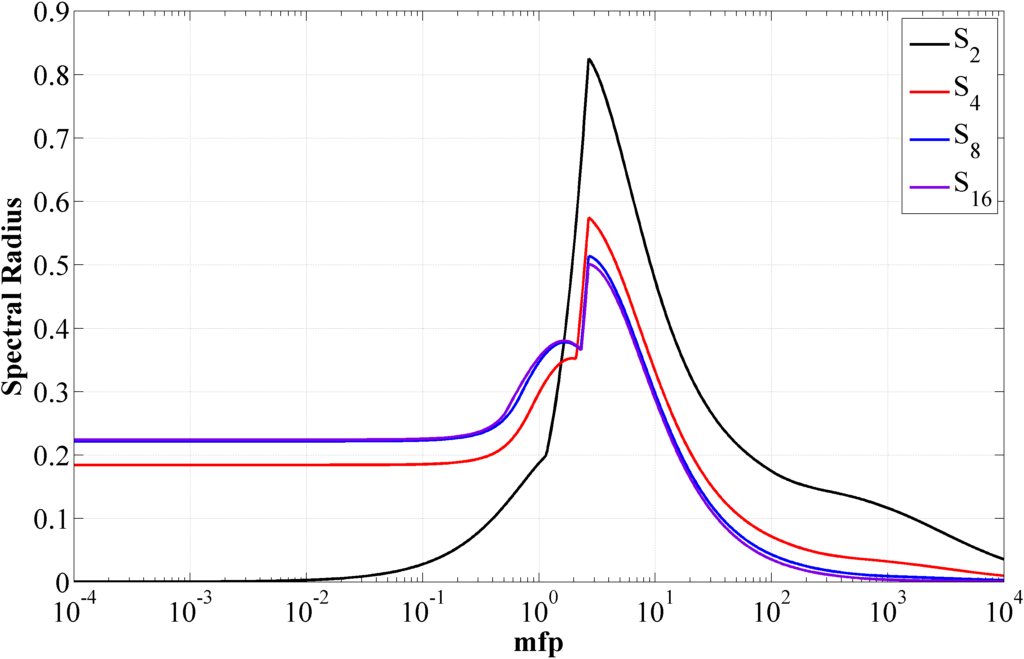
\includegraphics[width=\textwidth]{figures/appendices/DSA_1D_SI_MIP_C=1.png}
\caption{Spectral radius for the 1D MIP form using $c=1$.}
\end{figure}

\begin{figure}
\label{fig::1D_MIP_c=2}
\centering
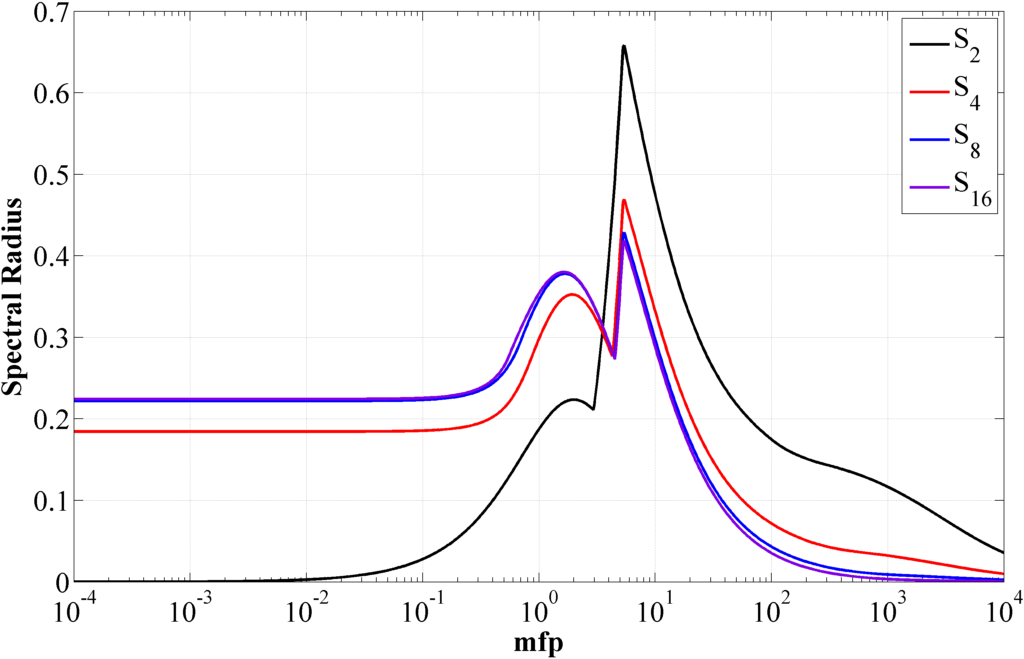
\includegraphics[width=\textwidth]{figures/appendices/DSA_1D_SI_MIP_C=2.png}
\caption{Spectral radius for the 1D MIP form using $c=2$.}
\end{figure}

\begin{figure}
\label{fig::1D_MIP_c=4}
\centering
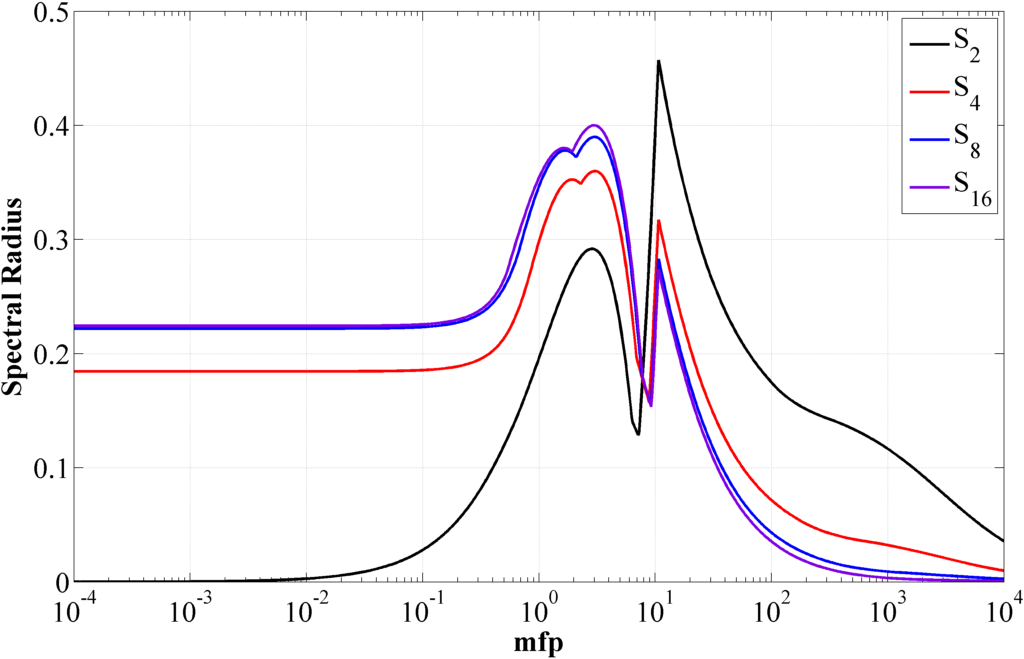
\includegraphics[width=\textwidth]{figures/appendices/DSA_1D_SI_MIP_C=4.png}
\caption{Spectral radius for the 1D MIP form using $c=4$.}
\end{figure}

\begin{figure}
\label{fig::1D_MIP_c=8}
\centering
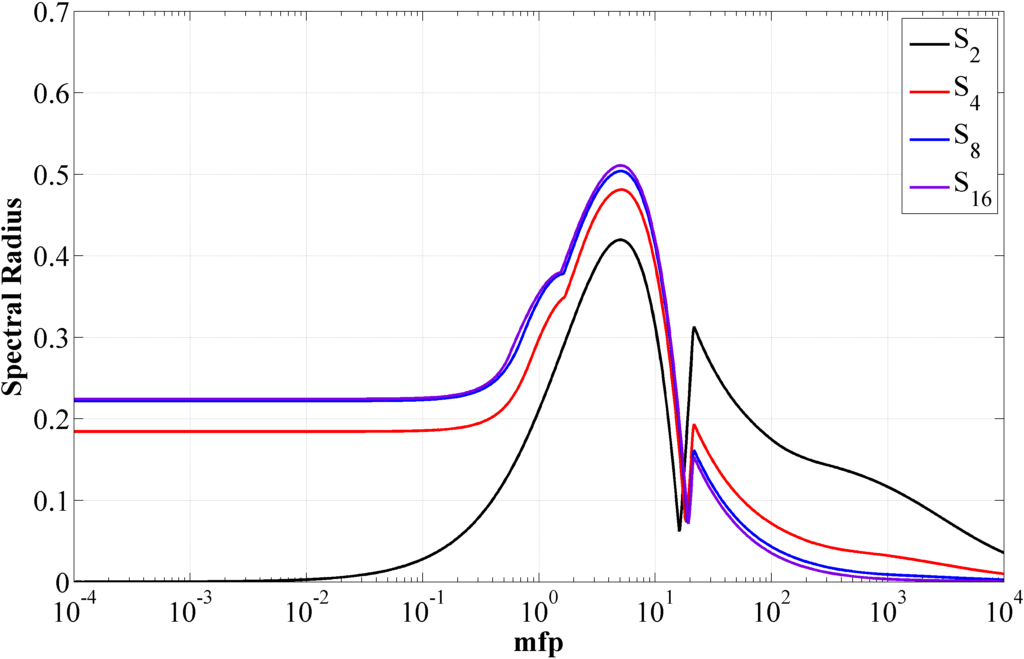
\includegraphics[width=\textwidth]{figures/appendices/DSA_1D_SI_MIP_C=8.png}
\caption{Spectral radius for the 1D MIP form using $c=8$.}
\end{figure}

\begin{figure}
\label{fig::1D_MIP_c=64}
\centering
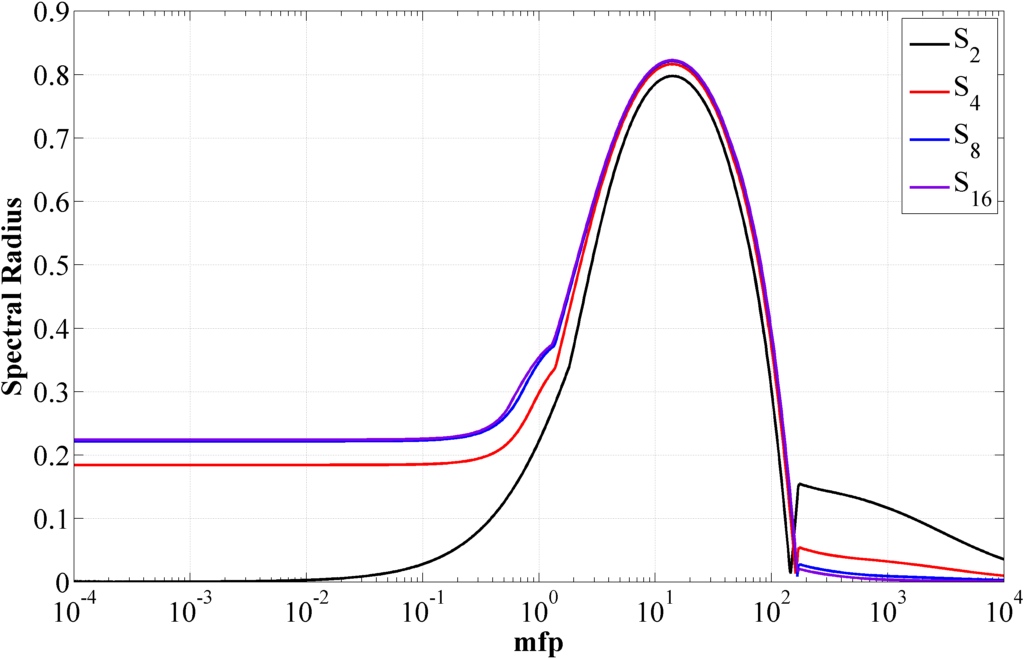
\includegraphics[width=\textwidth]{figures/appendices/DSA_1D_SI_MIP_C=64.png}
\caption{Spectral radius for the 1D MIP form using $c=64$.}
\end{figure}

\begin{figure}
\label{fig::1D_MIP_c=256}
\centering
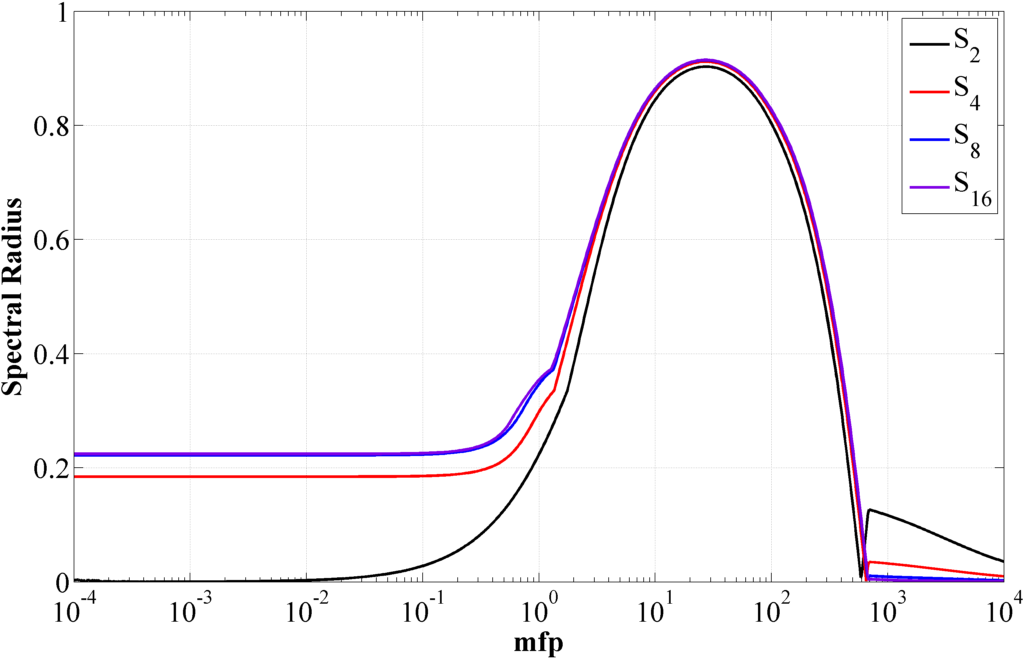
\includegraphics[width=\textwidth]{figures/appendices/DSA_1D_SI_MIP_C=256.png}
\caption{Spectral radius for the 1D MIP form using $c=256$.}
\end{figure}
% End: IP and MIP 1D Fourier Plots
%%%%%%%%%%%%%%%%%%%%%%%%%%%%%%%%%%%%%%%%%%%%%%%%%%%%%%


